\section{Motor Controller Unit}
\label{sec:MCU}
The purpose of the Motor controller unit(MCU) is to implement the motor driving algorithm. It also serves as the logger for the system, receiving data from BMS and logging data onto a SD-card. 

The chosen microprocessor is the PSoC 5LP(low power). This chip is placed onto a prototyping board with the name 'CY8CKIT-059 PSoC5LP Prototyping kit'.\fxnote{Husk ref}

\subsection{Design}

Figure \vref{PSoC} shows the connections associated with MCU. 

The PSoc in use come with a separate programmer, that can be snapped away. There must therefore be implemented an interface to program the PSoC when it is placed onto the PCB. This is realized by the 5x1 HDR as seen on figure \vref{PsoC}.

Capacitor C19 through C21 is capacitors needed by the internal structure of the PSoC. They are setup according to the datasheet and are needed by the ADC's being used. They are bypass capacitors required to ensure proper sampling at high sampling frequencies.

The PSoC is powered by the Distribution Block\vref{SMPS} where it receives 5V. This is within the input limits of the PSoC which ranges from 3.3V to 5V. Here it is being decoupled with a capacitor.  

The remaining connections at use are all the external interfaces to various items the board. This include both inputs and outputs from the PsoC. 

\begin{figure}[H]
	\centering
	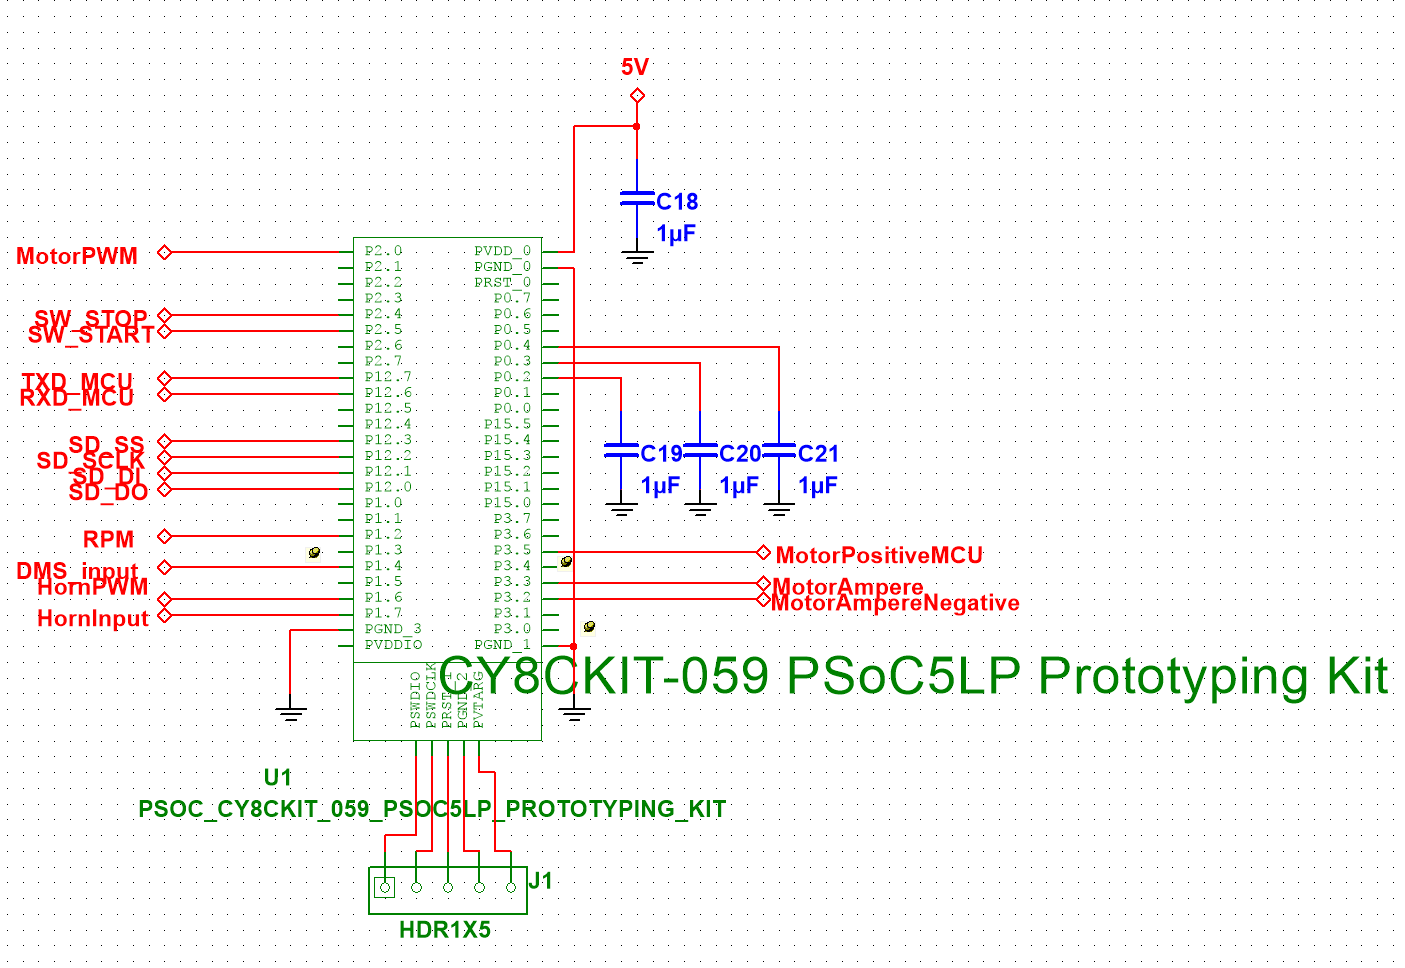
\includegraphics[width=0.7\linewidth]{Hardware/Pictures/PSoC}
	\caption{PSoC connections}
	\label{fig:PSoC}
\end{figure}

